\section{End-to-end LLM inference using Duplex}
\label{sec:duplex_llm_inference}



\subsection{Processing MoE and Attention Layers Using \lowp}
\label{sec:duplex_operation_logic_pim}
We propose a method for distributing computations assigned to each device across \lowp stacks. 
Fig.~\ref{fig:duplex_job_distribution} illustrates how the computations for the MoE and attention layers of decoding sequences are divided into four \lowp stacks. 
For the expert FFNs in an MoE layer, assigning a different expert to each \lowp could lead to varying execution times across \lowp due to differences in the number of tokens processed by each expert. 
We distribute each expert FFN computations across all \lowp for load balancing across \lowp.
However, this approach may necessitate inter-\lowp communication to obtain the final results. 

To minimize communication, we first distribute the weights for gate-projection and up-projection by slicing them column-wise across all \lowp. 
Since gated activation is an element-wise operation, it can be performed without additional data movement. 
Afterward, when computing down-projection, each \lowp ends up holding partial sums of the final output of the expert FFN. 
Performing an all-reduce operation among the \lowp within the device yields the final result of the expert FFN. 
This all-reduce operation is processed by an \highp, which reads and processes all the partial sums stored in the memory of each \lowp.
We minimize communication overhead by conducting a single all-reduce operation after all expert FFNs have completed their computations, rather than performing it after each expert FFN.


\duplex uses request and head parallelism for attention operations. 
Because attention operations among different requests have no data dependency, requests can be fully parallelized. 
As each head operates on separate slices of the Q vector and KV matrices, heads can also be fully parallelized.


\begin{figure}[!tb]
  \center
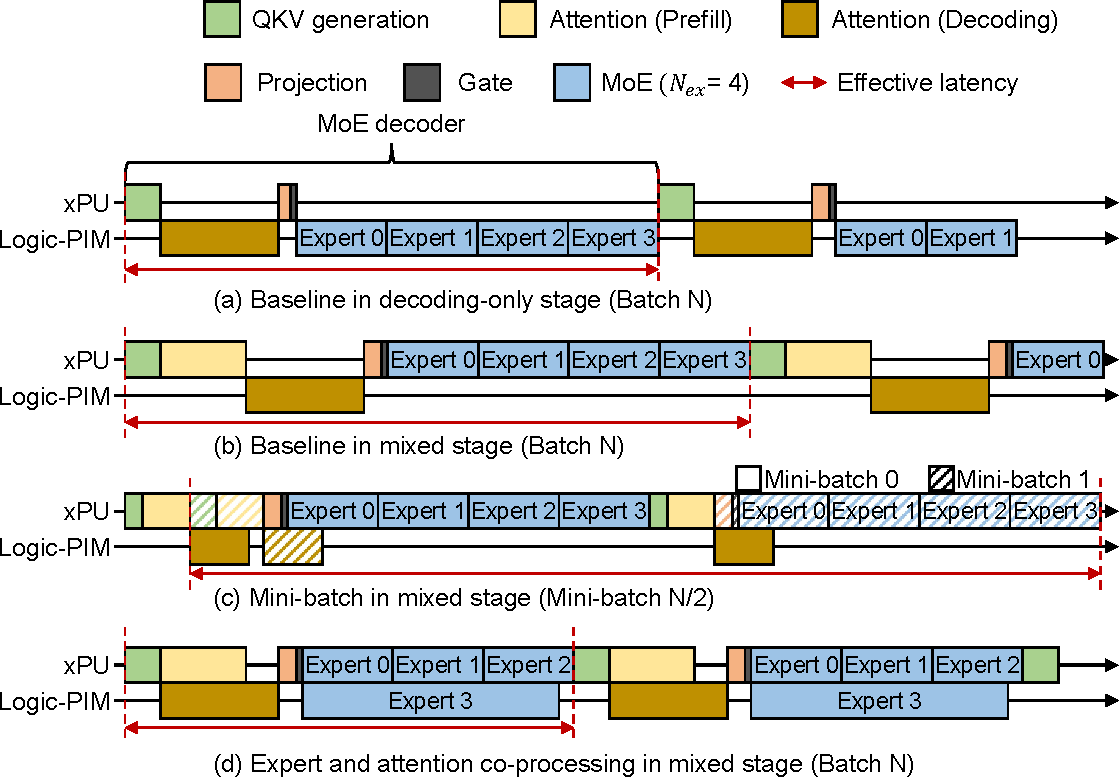
\includegraphics[width=1.00\columnwidth]{figures/operation_flow.pdf}
  \vspace{-0.13in}
  \caption{
  Operation flows of \duplex. Comparison of (a)--(d) for the same total batch size (N) with the same capacity of KV cache, considering the total device memory capacity. For convenience, the \deconlystage is depicted at a larger scale compared to the \mixedstage.
  }
  \label{fig:duplex_operation_flow}
  \vspace{-0.12in}
\end{figure}


\subsection{Expert and Attention Co-processing}
\label{sec:duplex_co-processing}
To increase the utilization of \highp and \lowp, we propose expert and attention co-processing.
In LLM inference, the presence of data dependencies between layers makes simultaneous computation in xPU and Logic-PIM challenging. 
Fig.~\ref{fig:duplex_operation_flow}(a) and (b) illustrates a na\"ive operation flow where only an \highp or \lowp is used at any given time. 


One simple way to simultaneously utilize \highp and \lowp is by dividing the workload into two independent mini-batches that have no data dependencies between them (Fig.~\ref{fig:duplex_operation_flow}(c))~\cite{asplos-2024-neupim}. 
These mini-batches enable simultaneous operations in xPU and Logic-PIM by alternating between layers, but it has disadvantages. 
The batching effect is reduced for the FC and MoE layers as these layers operate with half the batch size compared to the baseline method, leading to decreased data reuse. 
While attention operations are unaffected because each request processes independent values, the FC and MoE layers see no reduction in execution time when their operations are memory-bound, even with a reduced batch size. 
This can lead to increased latency compared to the baseline. 
Moreover, processing the same batch size doubles the amount of model parameters being read, resulting in higher DRAM read energy.



We propose expert and attention co-processing to increase the utilization of both processors, while maintaining the batching effect of the FC and MoE layers.
Expert FFNs in MoE layers do not have data dependencies between them, enabling simultaneous computation.
Because all tokens independently pass through a gate to select experts, the number of tokens processed by each expert can vary.
Experts with relatively fewer tokens are processed in \lowp, while the rest are handled in \highp in both \deconlystage and \mixedstage, thus preserving the batching effect of MoE layers while reducing its latency.



Because the number of tokens processed by each expert is determined after passing through gates, selecting which experts to process on each device may incur overhead. 
\duplex must decide which experts to allocate to either \highp or \lowp based on the time to process each expert with how many tokens are processed with each processing unit.
To minimize overhead, \duplex preliminarily estimates and stores the processing times for experts in both \highp and \lowp, depending on the number of processed tokens. 
At runtime, \duplex uses this lookup table to determine which experts to process in \lowp. 
First, \duplex calculates the total time to process all experts using only \highp.
Then, it progressively assigns the experts with the fewest tokens to \lowp, aiming to find the best combination for processing experts.
Then, \highp sends PIM instructions to \lowp to process the corresponding experts.
This lookup table-based decision-making is considerably faster than the actual execution of the expert layer, and its time impact can be considered negligible.

Using expert parallelism may diminish the impact of expert co-processing. 
With fewer experts processed in each device, the degree to which they can be split between xPU and Logic-PIM is limited, reducing the effectiveness of expert co-processing. 
Thus, we choose to apply tensor parallelism for MoE layers, splitting each expert across all devices. 
In the multi-node system, where the bandwidth between nodes is relatively lower than within the same node, we use expert parallelism between nodes and tensor parallelism within nodes.



Second, the mixed stage involves processing attention for both the decoding sequences and the prefilling sequences. 
As attention operations can be processed individually for each request, the attention of prefilling sequences is handled by the \highp, and that of decoding sequences is processed in \lowp, allowing us to process the attention layer more quickly.



\subsection{Memory Allocation and Management}
\label{sec:duplex_memory_space_allocation}
To support co-processing, we divide all the memory space in the device into four sections based on the index of the bank bundle. 
Each memory space uses bank bundles in all channels.
For the expert FFNs, we allocated them one by one across these four memory spaces. 
During expert co-processing, \duplex processes all the experts within the memory space with either \lowp or \highp, thus preventing any bank bundle conflicts between \lowp and \highp.

For the KV cache used in the decoding sequence, we have alternately allocated it among three of the memory spaces, while the remaining memory space is designated for storing Q, K, and V matrices used in the attention of prefilling sequences, thus enabling attention co-processing.
As the K and V matrices used in the prefilling sequences should be cached for the next stages, we need to migrate the K and V matrices to the other bank bundles for the next stage.
After the attention operation is finished, \highp moves the K and V matrices to the bank bundle designated to store KV cache.
Considering that this migration is performed only once, the overhead is negligible.
The parameters for the other layers are used exclusively in \highp and are allocated in any remaining memory spaces.